\section{Advection-Diffusion}
Before the implementation of the Nernst-Planck part of the model is
tested, a special case is considered, i.e. when the electrical
potential in the domain is constant. This makes the source term
including the electrical potential in eq. \eqref{nernst-planck} vanish
and we have to solve only for advection and diffusion.

Introducing characteristic scales for the concentration ($C_0$),
advective velocity ($u_0$) and length ($l_0$) respectively, gives the
non-dimensional advection-diffusion equation for incompressible flow:

\begin{equation}\label{non_dim_adv-dif}
\frac{\partial C}{\partial t} + \mathbf{u} \cdot \nabla C = 
\frac{D}{u_0 l_0} \nabla^2C.
\end{equation}

All variables in \eqref{non_dim_adv-dif} are non-dimensional. The
quantity $Pe = u_0l_0/D$ is often referred to as the P\'{e}clet number. It
determines the relation between contributions to the
dynamics from advection and diffusion respectively. For $Pe \gg 1$ the
dynamics is dominated by advection and for $Pe \ll 1$ by diffusion. 

The LB model described in section \ref{sec:nernst-planck_lb} was
tested by studying the evolution in time and space of a point mass in
one dimension. The analytical solution of eq. \eqref{non_dim_adv-dif}
in one dimension with initial conditions $C(x, t = 0) = \delta(x)$ on
an infinite domain is:

\begin{equation}
C(x, t) = \sqrt{\frac{Pe}{4 \pi t}}\exp\left({-\frac{(x - ut)^2
    Pe}{4t}}\right).
\end{equation}

In the numerical computations the parameters $Pe = 10$ and
$|\mathbf{u}| = 0.1$ were used. The domain consisted of 200 lattice
nodes and three snapshots in time at $t = 100, 200, 300$ were compared
to the analytical solution. The result is presented in
fig. \ref{fig:adv-dif}.

\begin{figure}\label{fig:adv-dif}
\begin{center}
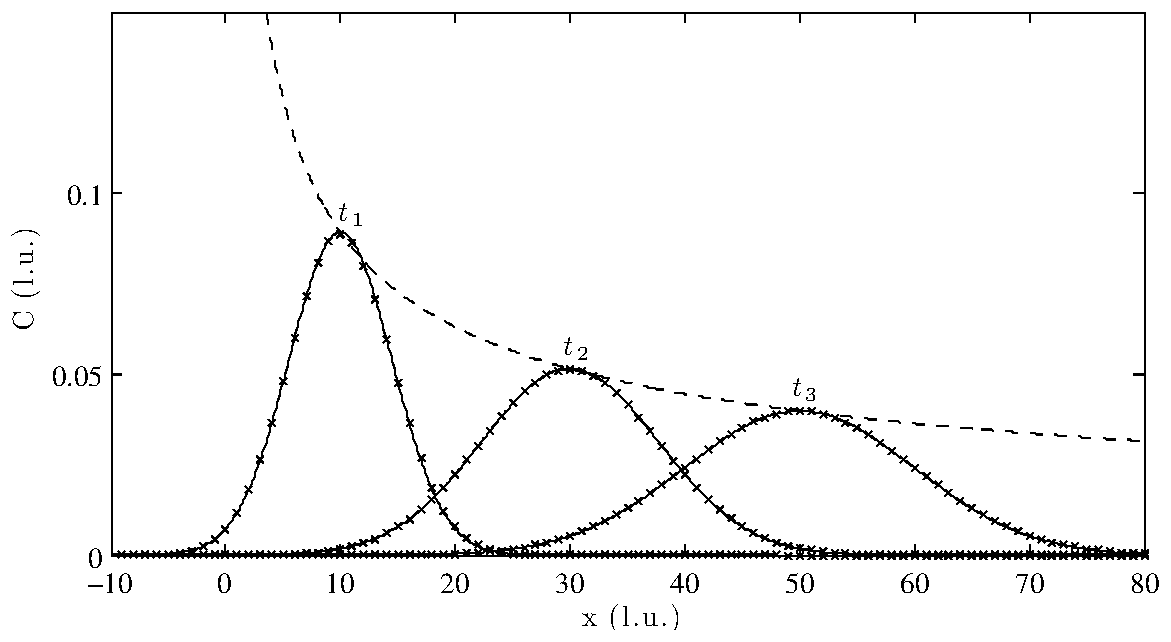
\includegraphics[width=0.9\textwidth]{fig/adv_dif_10_30_50.pdf}
\end{center}
\caption{Obtained solutions ($\times$) of the
  advection-diffusion equation for a point mass evolving in time and
  space. Three different times ($t_n = 100n$) are compared to
  analytical solutions (solid). The Amplitude of the solutions as
  function of time has also been plotted (dashed). The advecting
  velocity, $u_0 = 0.1$ and the Peclet number, $Pe = 10$.  All units
  are in lattice units.}
\end{figure}
